\documentclass{paper}
\usepackage{times}
\usepackage{geometry}
\geometry{letterpaper, portrait, margin=1in}
\usepackage{setspace} \doublespacing
%\usepackage{setspace} \singlespacing
\usepackage[utf8]{inputenc}
\usepackage{enumitem,amssymb}
\usepackage{ragged2e}
\usepackage{physics}
\usepackage{siunitx}
\usepackage{wasysym}
\sisetup{separate-uncertainty=true}
\usepackage{float}
\usepackage{mathtools}
\usepackage{amsmath}

\usepackage{caption}
\usepackage[hidelinks]{hyperref}
\usepackage{url}

\usepackage{graphicx}
\usepackage{epstopdf}
\usepackage{tikz}
\graphicspath{{data/concepts}}

\usepackage{aas_macros}
\usepackage[style=authoryear]{biblatex}
\bibliography{refs} %refs.bib
\nocite{*}

\immediate\write18{texcount \jobname.tex -out=\jobname.sum}

% set frameboxes to be borderless
\setlength{\fboxsep}{0pt}
\setlength{\fboxrule}{0pt}

\begin{document} 

\title{The constituents of the universe and the growth of structure}
\author{ariahayd}
\date{April 24, 2022}
\maketitle

% Overview. [8]
% Give an overview of the current standard model for the context of the essay. 
% Include one figure for this section. 
\section{Overview}
  The universe is shaped by its constituent energies, and its constituents are
  shaped by the scale of space. The evolution of the universe is understood 
  through the Standard Model of Cosmology, developed mainly over the last 
  century of observations of matter and energy on large scales, of galaxies 
  throughout cubic gigaparsec volumes space, and on the very small scales 
  where the quantum mechanical properties of energy fields emerge. 

  The most successful model is $\Lambda$CDM, the concordance model, with 
  dynamics explained through General Relativity and Quantum Field Theory, and 
  with contributions from dark energy ($\Lambda$) and cold dark matter 
  (CDM). These last two components are observationally confirmed but not 
  entirely explained by theory. 

  The densities of energy in the fields within the universe determine the 
  geometry of space. $\Lambda$CDM requires a universal geometry curved by 
  the energy densities of these constituent fields. Observations indicate that 
  the curvature of the metric of spacetime over large distances is nearly 
  flat and has been throughout most of the history of the universe.
  
  \begin{figure}[H]
    \begin{centering}
    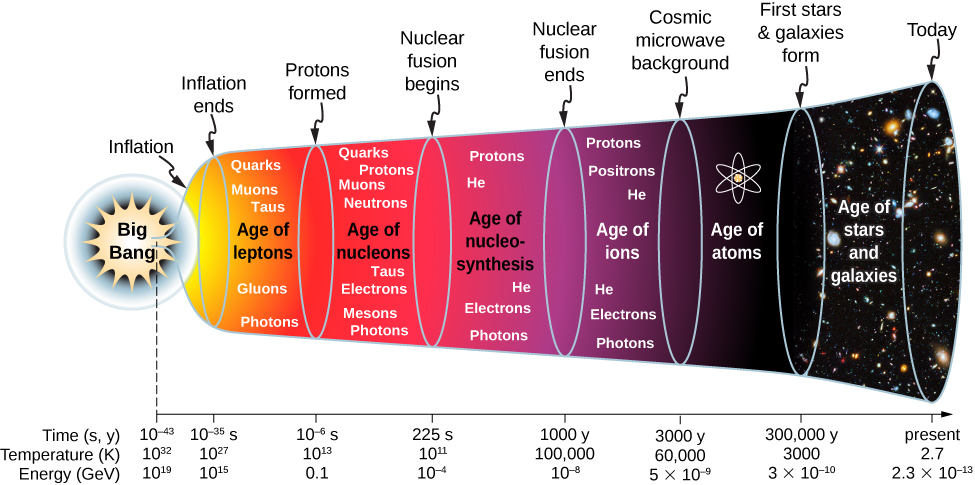
\includegraphics[scale=0.8]{Intro-big_bang.pdf}
    \caption{A timeline of the hot big bang with times for each epoch,
      along with the average temperature, and average energy per particle.
    Credit: \cite{2016Ling}}
    \label{fig:Intro-big_bang}
    \end{centering}
  \end{figure}

  $\Lambda$CDM is based on a hot big bang origin of high energy density 
  that has since evolved to the today's universe of much lower density. 
  Principal evidence of a hot big bang is from the distribution of quasar 
  radio signals isotropically distributed throughout space, but all distant
  in time, indicating that the environments of galaxies were very different
  in the past (\cite{Secrest_2021}) and that the universe is not in an
  eternal steady state. 

  The standard model explains how energy fields latent in space express in 
  different ways at different points in evolutionary epochs, expanding the 
  scale of space in the inflationary and current epochs, and smoothing out the 
  distribution of gravitationally bound particles in the radiation dominated 
  era. An illustration of this timeline is shown in Fig. 
  \ref{fig:Intro-big_bang}. The main successes of $\Lambda$CDM are 
  explanations of the origin of the abundances of observable matter and 
  primordial photons in the universe that come from these fields.

  A hot big bang can be derived from an analysis of the metric of spacetime 
  applied to a homogeneous universe combined with observations of the isotropic
  recession of luminous objects. The assumption that the total volume of 
  the universe holds a finite energy implies a positive curvature to space and
  an eventual collapse under self-gravitation. That the collapse has not 
  happened, and to force a long term steady-state to the geometry of the 
  universe, led the original authors to include a $\Lambda$ term in the 
  cosmology (\cite{10.1093/mnras/90.7.668}). The standard model today is based 
  on the same terms, but explains the detail through different physics on
  small and large scales, on the scale of particles to galaxies clusters.

% 2. Dark Matter. [20]
% Describe two lines of evidence for dark matter. These should be distinct and 
% complementary. A line of evidence can consist of more than one observational 
% phenomenon that together provide the evidence. Include two figures for this 
% section.
\section{Dark Matter}
  Large, gravitationally bound systems such as galaxies and galaxy clusters 
  appear to be embedded in gravitational potentials deeper than expected given 
  the observable masses interacting within the system. The depth of these 
  potentials is inferred to be due to unobserved, \textit{dark} matter.

  % line of evidence one
  Early evidence for dark Matter in the halo of a galaxy comes from
  measurements of the rotational velocities of the material in the arms of
  spiral galaxies. A spiral galaxy is a stable, virialized structure bound by
  gravity and is expected to follow the Newtonian gravitation model for a
  fluid rotating around a center mass. The spiral arms are not coherent
  structures in themselves, but are the result of a density way propagating 
  through the fluid hydrodynamics of the galactic disk. 

  The rotational velocity of the disk can be estimated via the 
  width of the HII emission lines across the disk of the galaxy, as was done
  for M31 (\cite{1970ApJ...159..379R}), showing the velocity field follows a 
  profile more like a solid body rotating around a center mass than a fluid 
  swirling around a core. Because the dynamics of galaxies can indeed be 
  modeled as a fluid, the only explanation for a velocity field continuing 
  beyond the visible matter of the galaxy is for an unobservable mass 
  encircling the galaxy in a spherical halo.

  \begin{figure}[H]
    \begin{centering}
    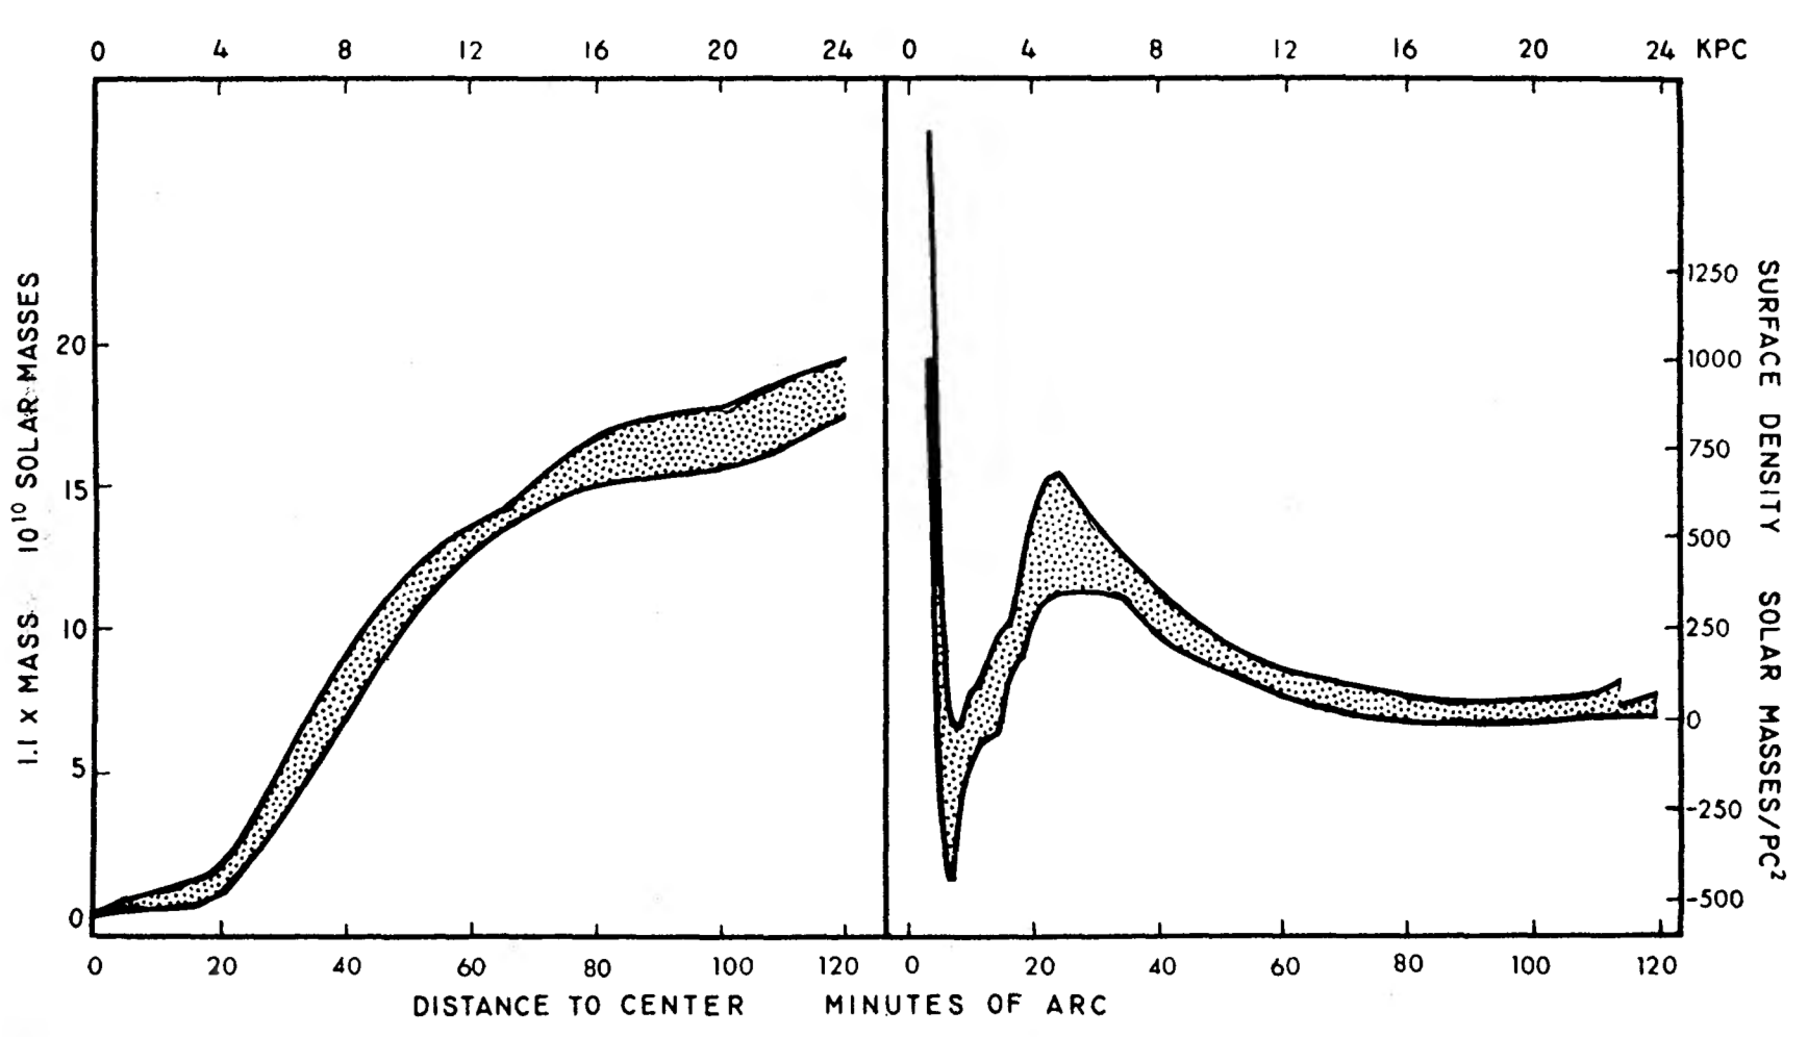
\includegraphics[scale=0.4]{DM-masscurve.pdf}
    \caption{Fourteen different mass models fitting the velocity map data of
      M31 are combined to yield a band of mass estimates, on the left, and 
      surface densities, on the right, from the center to beyond the luminous 
      edge of M31, a galaxy considered to have an has an apparent angular 
      diameter of \SI{178}{arcsec}.
      Credit: \cite{1970ApJ...159..379R}}
    \label{fig:DM-masscurve}
    \end{centering}
  \end{figure}

  The projected mass sheets of these halos are responsible for strong and weak 
  gravitational lensing that can be observed abound massive cosmic 
  structures.  Since these early observations, dark matter halos have been 
  measured for most bound systems on the scale of galaxies or clusters, though 
  there is also evidence of anomalous galaxies that may lack a significant 
  concentration of dark matter around them (\cite{10.1093/mnras/stab3491}). 

  Halos have been demonstrated to move with core material of galaxies and not 
  with energetic plasma that makes up majority of baryonic mass in a galaxy when 
  the plasma is disrupted and ram-pressure stripped out of the galaxy. 
  Dark matter is bound to the gravitational potential of the galaxy rather 
  than to the baryons in the potential (\cite{Clowe_2006}). This observation 
  reinforces the ``cold'' nature of dark matter; that it cannot kinetically 
  escape the potential that also binds baryonic masses, and indicates that it 
  is decoupled from interactions with baryons. 

  %line of evidence two
  That dark matter could not be contributed entirely by baryonic particles
  has been clear since the 1980s (\cite{liddle2015introduction}) when
  solutions to the hot big bang model during the radiation era showed that 
  pressure waves traveling through the irradiated plasma would damp the
  accretion of the baryonic matter in any potential wells evident in the 
  anisotropy signal of spherical harmonic modes in the cosmic microwave 
  background measurements.

  The baryon acoustic oscillation signal comes from modeling the destructive
  interference pattern of the coupled photon-baryon fluid that permeated the
  radiation-dominated era of the universe. The restoring force of a pressure
  variance in this fluid comes from the ionization and scattering between
  primordial atoms and photons interacting frequently due to the overwhelming
  prevalence of high energy photons resulting from baryogenesis, as most 
  baryons annihilated with their anti-particle pair, converting to photons.

  Gravitational fluctuations must have been built prior to the decoupling and 
  could not have been solely due to density variations in the photon-baryon 
  fluid.  There must have been a dark matter component to the ``frozen'' into 
  the environment of the plasma, seeding the gravitational fluctuations that 
  would quickly accrete material after decoupling, forming galaxies and the 
  first luminous objects. As shown in Fig. \ref{fig:DM-BAO}, the number 
  density of galaxies in volumes of space, measured through redshift survey, 
  correlates to the baryonic acoustic oscillation signal at the scale of an 
  earlier period in the universe.

  % \cite{2007MNRAS.381.1053P}
  
  % How small were the first cosmological objects?
  %The minimum baryonic mass that can become virialized is a function of \(z\),
  %from \SI{E6}{\astrosun} at \(z=15\) 
  % \cite{1997ApJ...474....1T}

  Explanations of dark matter can be categorized two ways; either due to 
  massive, compact halo objects (MACHOs) or by weakly interacting massive 
  particles (WIMPs). Searches for MACHOs, large, bound bodies in a galactic 
  halo, have returned no significant findings. Though dark matter can be 
  observed through phenomena understood through the standard model, there is 
  no candidate WIMP particle that could constitute dark matter in the standard 
  model. An explanation of the WIMP contribution to dark matter as something 
  like a primordial, massive graviton, requires new physics.
  (\cite{PhysRevLett.128.081806})

  \begin{figure}[H]
    \begin{centering}
    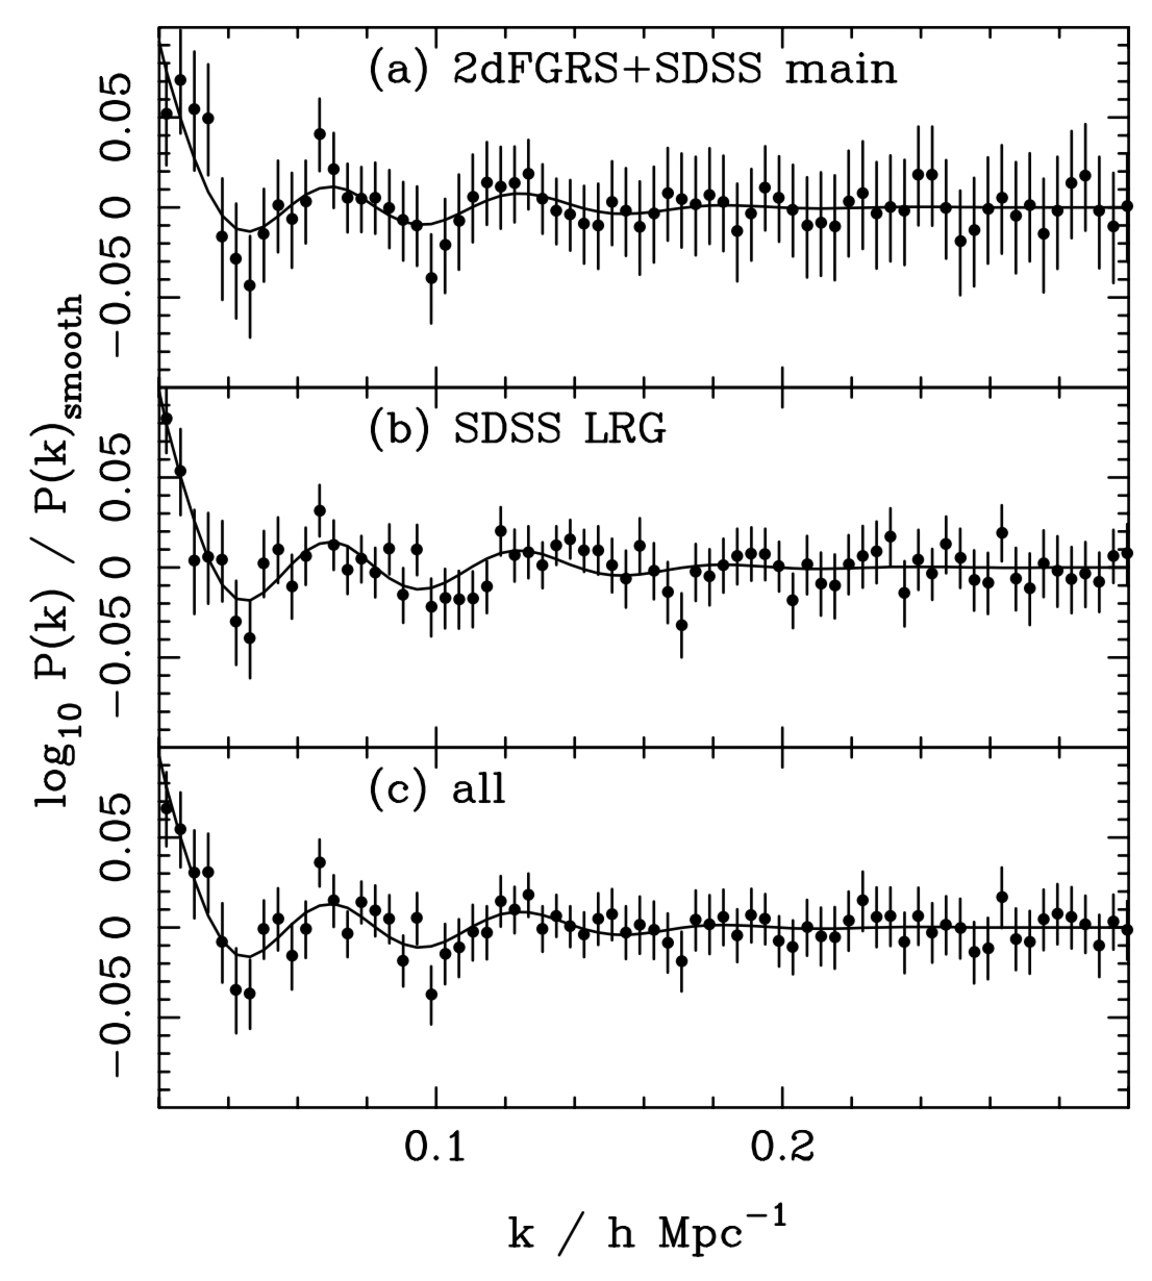
\includegraphics[scale=0.6]{DM-BAO.pdf}
    \caption{A combination of two galaxy surveys show the correlation of
      the density of galaxies with modeled density distribution from the
      baryon acoustic oscillation wave modes in the coupled photon-baryon
      fluid of the radiation dominated era. $k$ is the wave number of the
      the oscillating pressure wave. \(h = 0.7\) is the dimensionless Hubble
      constant. These observations match a model with a total energy density
      due to matter, \(\Omega_m = 0.25\), while the baryonic contribution is
      observed to be \(\Omega_b = 0.05\), indicating that the 
      difference is dark matter (\cite{Eisenstein_2005}).
    Credit: \cite{2007MNRAS.381.1053P}}
    \label{fig:DM-BAO}
    \end{centering}
  \end{figure}

% 3. Baryons. [20]
% Describe one indirect constraint on the baryon density (BBN or CMB), and key 
% direct measurements of various baryonic components. Include two figures for 
% this section.
\section{Baryons}
  Constraints on the density of baryons among the energies of the universe are
  based on modeling the prevalence of atoms generated during the big bang 
  nucleosynthesis era or by modeling angular size of spherical harmonic 
  patterns in the surface of last scattering of the decoupling event. Both 
  approaches for constraining the baryonic contribution to the matter density 
  are indirect because the methodologies infer the baryonic prevalence from 
  understood physics at early times rather than from direct measurements.

% That primordial chemical elements would have been produced in the 
% environment of a hot big bang, and that the duration of expansion rather 
% than temperature would determine the prevalence of elements, was theorized 
% (\cite{PhysRev.73.803}) before the term ``big bang'' was coined 
% (\cite{Hoyle1949}) and well before the debate over a big bang or continuous 
% creation origin had been decided.

  Particles coalesced in at least four early epochs. The end of the first era,
  the X-boson era, at \SI{E-38}{s}, fixed the baryon and lepton number. 
  In the second, the Quark-Hadron era, quarks combined to form the baryonic 
  nucleons. This era ends at \SI{E-6}{s} with an asymmetry between baryonic
  particle and antiparticle pairs, in which baryons are estimated with an 
  excess of \SI{E-9} per pair (\cite{1993PhRvL..70.2833F}). The third, the 
  Lepton Era, ends at \SI{1}{s} as the temperature decreases to the point 
  where neutrinos are no longer coupled to electron-positron pairs, and can 
  escape reactions. Throughout these eras, WIMPs are expected to have been 
  present in the background contributing to local density fluctuations 
  through gravitation, but not through interactions.

  The fourth epoch, the Nucleosynthesis Era, between \SI{1}{s} and 
  \SI{300}{s}, was the duration over which weak force interactions changed
  the number distribution of protons and neutrons and then primordial atomic 
  nuclides formed. The prevalence of free neutrons was constrained by both
  processes, and the resulting abundances of light elements throughout the 
  universe generally matches the Standard Big Band Nucleosynthesis (SBBN)
  prediction. SBBN is based on the foundational physics of $\Lambda$CDM 
  during the radiation dominated era and the inclusion of three neutrino 
  species (\cite{Cyburt_2016}). 

  Weak interactions maintained the balance of protons and neutrons early in
  the Nucleosynthesis Era until the declining temperature of the fluid reduced 
  the likelihood of producing the neutron, slightly heavier than the proton, 
  in the balance of the reactions. At \(T = \SI{E10}{K}\) the fraction of 
  neutrons to all baryons freezes at \(18\%\). This represents the neutron 
  budget for nuclear reactions that produce primordial atomic nuclei, a budget
  declining exponentially over the next \SI{886}{s} following the 
  characteristic timescale for the decay of free neutrons through \(\beta\)
  emission.

  Atomic nuclei do not grow through many-body reactions among participating
  baryons because the cross section of interaction for the specific particle
  ingredients needed to form a nucleus is rare. Instead, nuclei are built
  through a chain of two-body reactions. The first reaction in the chain
  combines a proton with a neutron to form deuterium. However, a deuterium
  nucleus is not tightly bound and is easily broken back into constituent
  particles by interactions with photons until the temperature drops to 
  \(T = \SI{E9}{K}\) at \(t = \SI{300}{s}\). After this point in cooling, 
  deuterium nuclei are available to form \(\prescript{3}{}{He}\), 
  \(\prescript{4}{}{He}\), \(\prescript{6}{}{Li}\), \(\prescript{7}{}{Li}\), 
  and \(\prescript{7}{}{Be}\) through chains that reach equilibrium on
  timescales shown in Fig. \ref{fig:BBN-frac}.

  \begin{figure}[H]
    \begin{centering}
    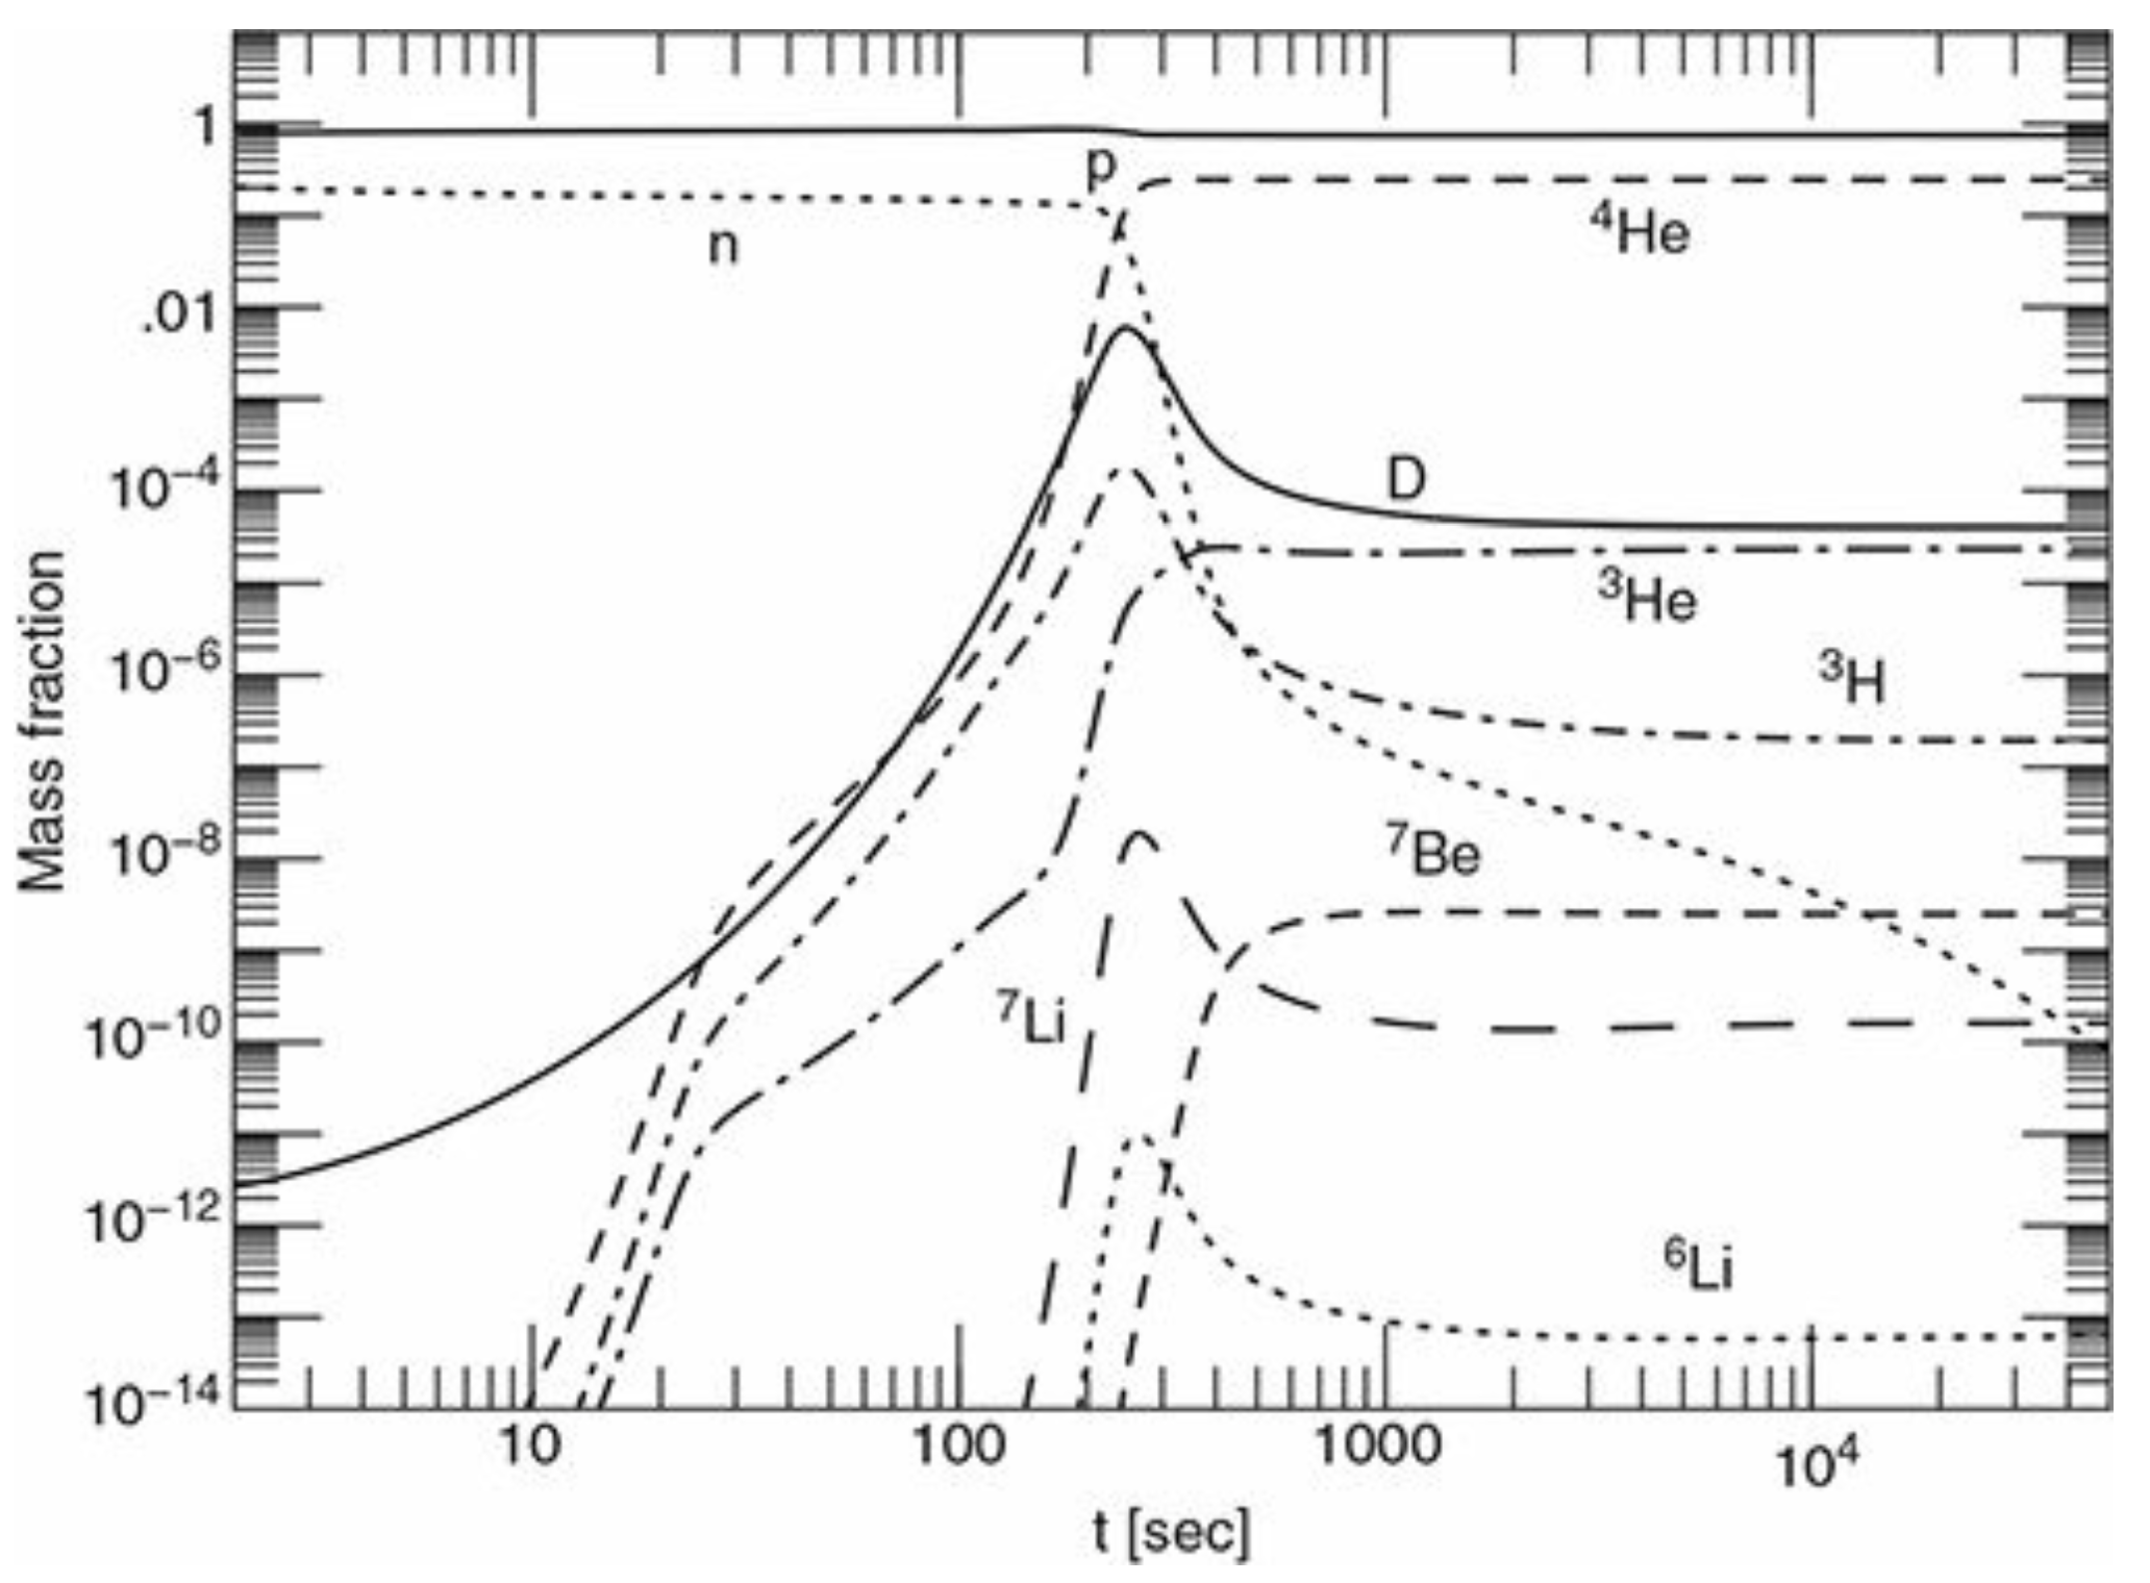
\includegraphics[scale=0.4]{BBN-frac.pdf}
    \caption{A chart of the mass fraction of baryons and nuclides over the
      SBBN era. Note that the fraction of protons remains essentially static
      while neutrons are consumed to make nuclides. The mass fraction of 
      neutrons declines overall, but drops precipitously after 
      \(t = \SI{200}{s}\) as the neutron number fraction among baryons froze 
      and the characteristic lifetime of unbound neutrons allowed rapid decay.
      Scales are in log. The mass fractions of primordial nuclides heavier
      than \(\prescript{4}{}{He}\) are vanishingly small.
    Credit: \cite{ryden2003introduction}}
    \label{fig:BBN-frac}
    \end{centering}
  \end{figure}

  Measuring the metal content of stars in the least active globular clusters, 
  which are assumed to be the best preserved early environments that can be 
  observed nearby, approximates but does not exactly match the predicted 
  abundances of SBBN atoms. This indicates some stellar processing prior to 
  the oldest clusters. Using clusters as ``chronometers'' suggests a time 
  since the big bang of \SI{15.6(46)E9}{years} (\cite{1999ApJ...521..194C}).

  %baryongensis is a process that violates CP conservation
  %In the standard model of cosmology, baryon number is not conserved
  %(\cite{PhysRevLett.37.8}). From the
  %(\cite{DINE1991351})

  \begin{figure}[H]
    \begin{centering}
    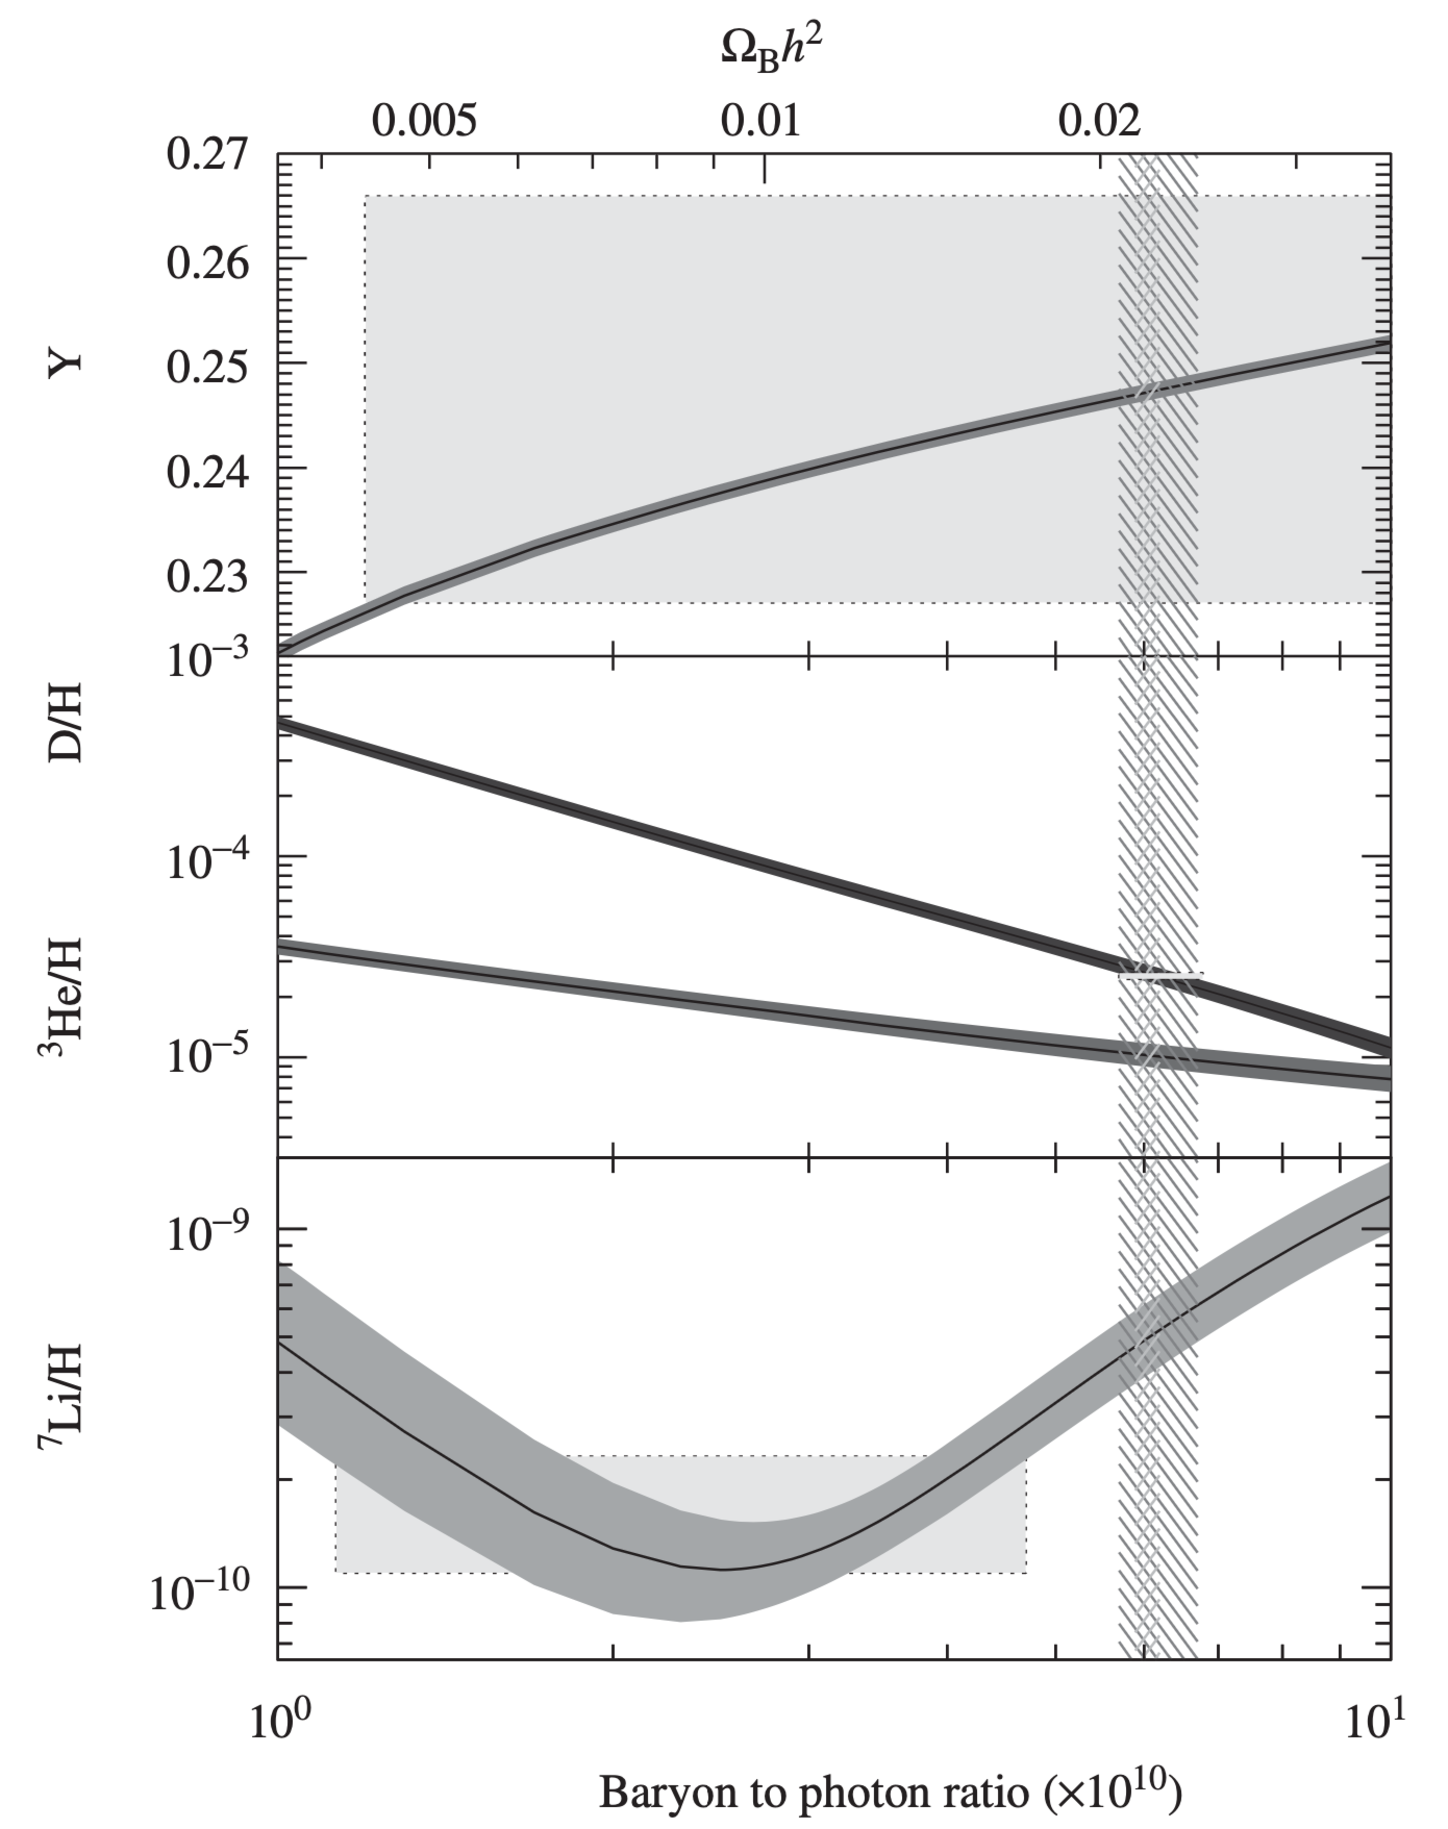
\includegraphics[scale=0.5]{BBN-ratios.pdf}
    \caption{A modeled prediction of the abundances of nuclides through big
      bang nucleosynthesis assuming a neutron characteristic lifetime of
      \(\tau_n = \SI{880.3(11)}{s}\) and a neutrino species number of 3. 
      \(Y\) is the fraction of primordial \(\prescript{4}{}{He}\). The width 
      of each band is related to the uncertainty in the cross-section of 
      interaction for each nuclear species. Boxes in the figure are values 
      allowed by observations. The vertical striped band is the constraint 
      based on observations of deuterium, limiting 
      \(0.043 \leq \Omega_b \leq 0.051\), while the crosshatched band 
      is the inference of \(\Omega_b\) from the cosmic microwave 
      background.  Note that values for \(\prescript{7}{}{Li}\) do not match 
      observation. The baryon to photon ratio is a range of excess photons
      resulting from baryon pair production.
      Credit: \cite{liddle2015introduction}}
    \label{fig:BBN-ratios}
    \end{centering}
  \end{figure}

  Most of the baryons in the universe, 75\%, are not gravitationally bound in 
  structures like galaxies, but are diffuse in the intergalactic medium. By 
  measuring the dispersion, the delay in repeated signaling of fast radio 
  bursts through a modeled column of electrons relative to a true vacuum with 
  no particles to scatter the photons, the unbound baryonic matter has been 
  measured at \(\Omega_b = 0.051\) (\cite{2020Natur.581..391M}).

  %Correlation function galaxy distribution as constraint on DE
  % \cite{2003ApJ...594..665B}

% 4. Dark Energy. [20]
% Describe two lines of evidence for dark energy. Comment on possible 
% modifications to the standard model. Include two figures for this section.
\section{Dark Energy}
  The energy density of the universe seems to be driven to the critical 
  density that results in flat spatial metric, even at points in the
  the standard model evolution of the universe in which it could be expected
  to deviate away from the critical density due to the shaping effects of 
  energy densities.

  The pressure nudging spacetime to a flat curvature in the current epoch is 
  known as dark energy, the $\Lambda$ component of the $\Lambda$CDM
  model, because the source of energy has not yet been fully explained. 
  It is though to be a constant, latent energy density of the vacuum of 
  spacetime in a phase above a potential ground state.

  Evidence for dark energy in the $\Lambda$CDM model comes from two 
  significant observations that independently constrain the contribution of 
  $\Lambda$ to the energy budget, namely measurements of the recession of 
  supernovae as standard candles and measurements of the angular size of 
  standard rulers in the cosmic microwave background anisotropy.

  Fig. \ref{fig:DE-sn_lightcurve} is a Hubble diagram showing the redshift in
  spectrum of surveyed supernovae events. Assuming redshift to be a proxy for
  recession velocity, the data indicate that an increase in recession 
  velocity with distance from the observer, implying an acceleration between
  the positions of observation and event against the rest frame of a
  fundamental observer. The Supernova Cosmology Project, completed in 2011, 
  added ten more supernova events to the diagram (\cite{2012ApJ...746...85S}).

  % supernovae \cite{Riess_1998}
  \begin{figure}[H]
    \begin{centering}
    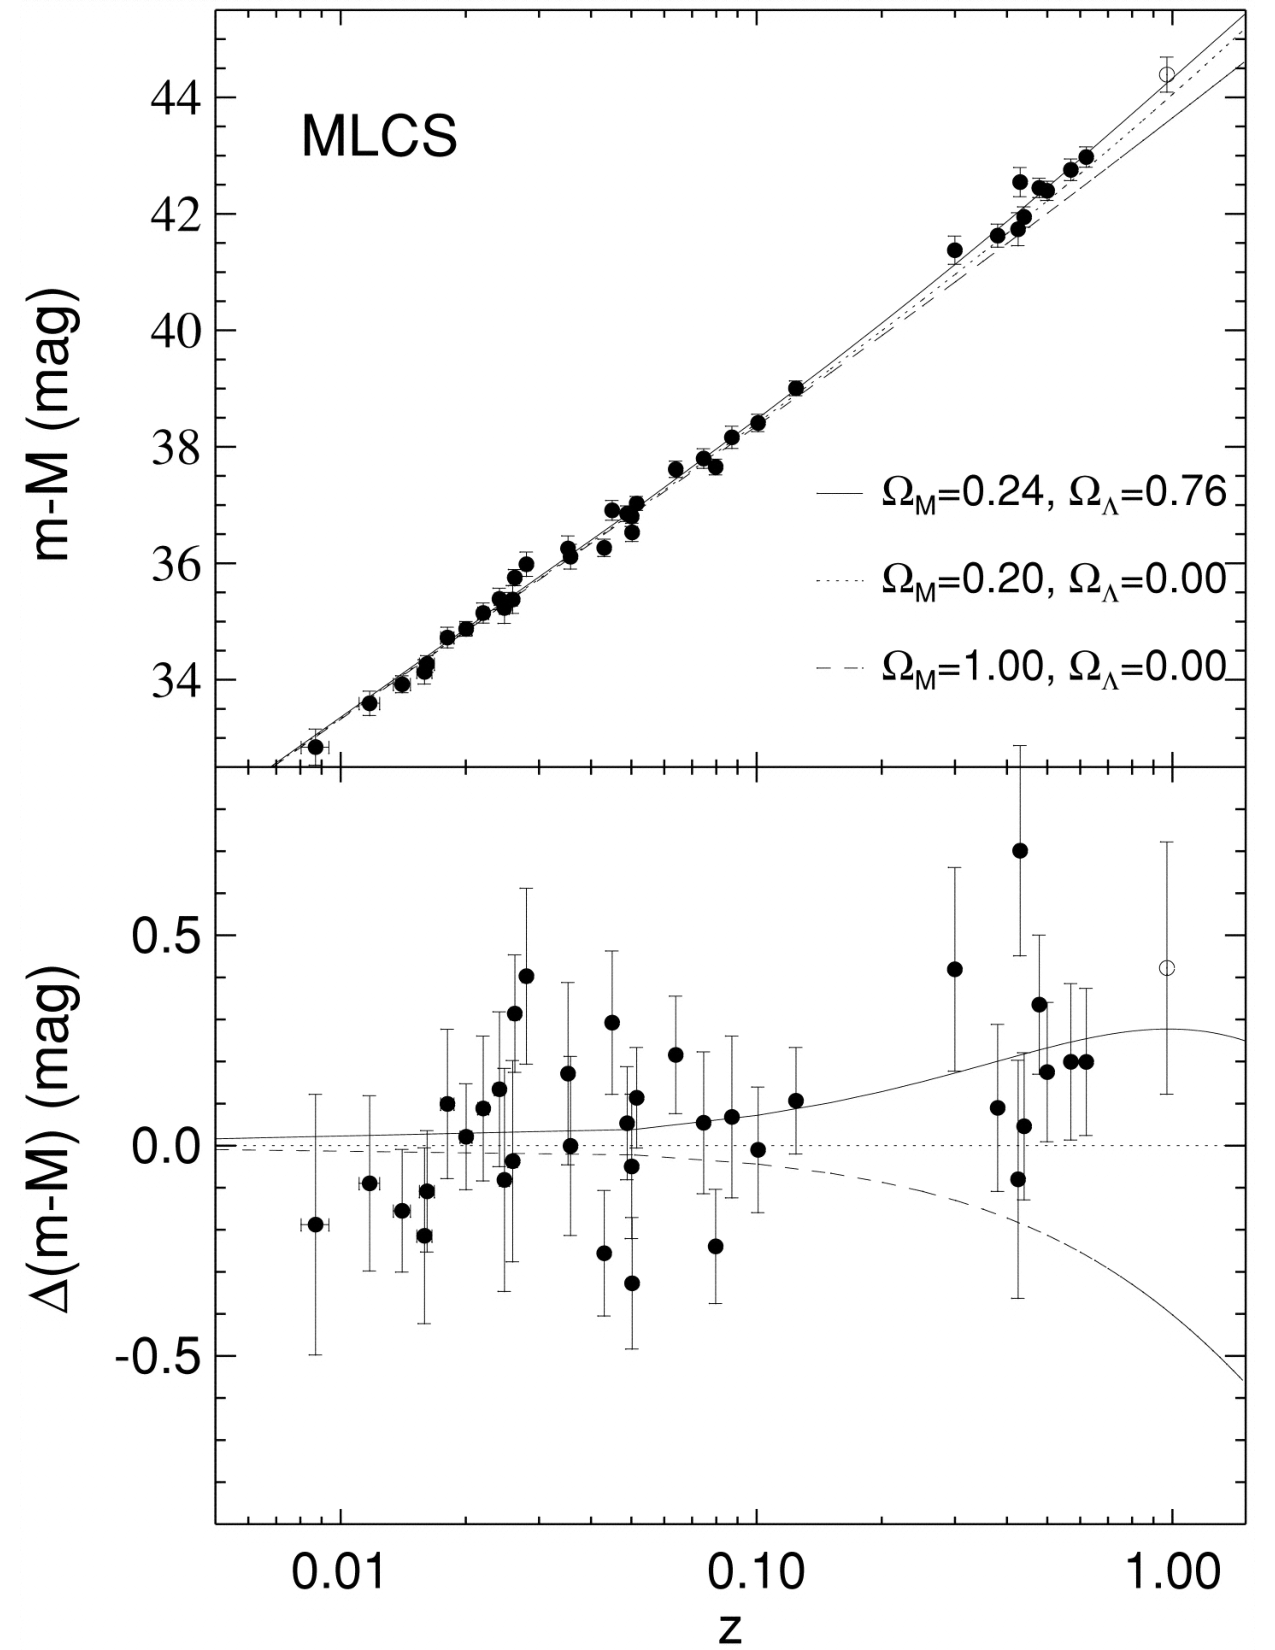
\includegraphics[scale=0.5]{DE-sn_lightcurve.pdf}
    \caption{The figure on the top is a fit of a measurement of the multicolor 
      light curve shape (MLCS) characteristic of SNe Ia as a function of 
      measured redshift of the event spectrum. The figure below is the
      difference between measured magnitude and modeled magnitude for an 
      environment with no dark energy, i.e. \(\Omega_{\Lambda} = 0\), to show
      that observations convincingly deviate from an \(\Omega_{\Lambda} = 0\) 
      environment.
      Credit: \cite{Riess_1998}}
    \label{fig:DE-sn_lightcurve}
    \end{centering}
  \end{figure}


% \begin{figure}[H]
%   \begin{centering}
%   \includegraphics[scale=0.6]{DE-constraints.pdf}
%   \caption{Constraints on the free parameters of the $\Lambda$CDM
%     model predicting a range of values for \(\Omega_{m}\) and 
%     \(\Omega_{\Lambda}\). The topographic lines of each parameter represent 
%     confidence intervals in the measurement. This figure excludes systematic
%     errors in the supernovae measurements.
%     Credit: \cite{2012ApJ...746...85S}}
%   \label{fig:DE-constraints}
%   \end{centering}
% \end{figure}

  \begin{figure}[H]
    \begin{centering}
    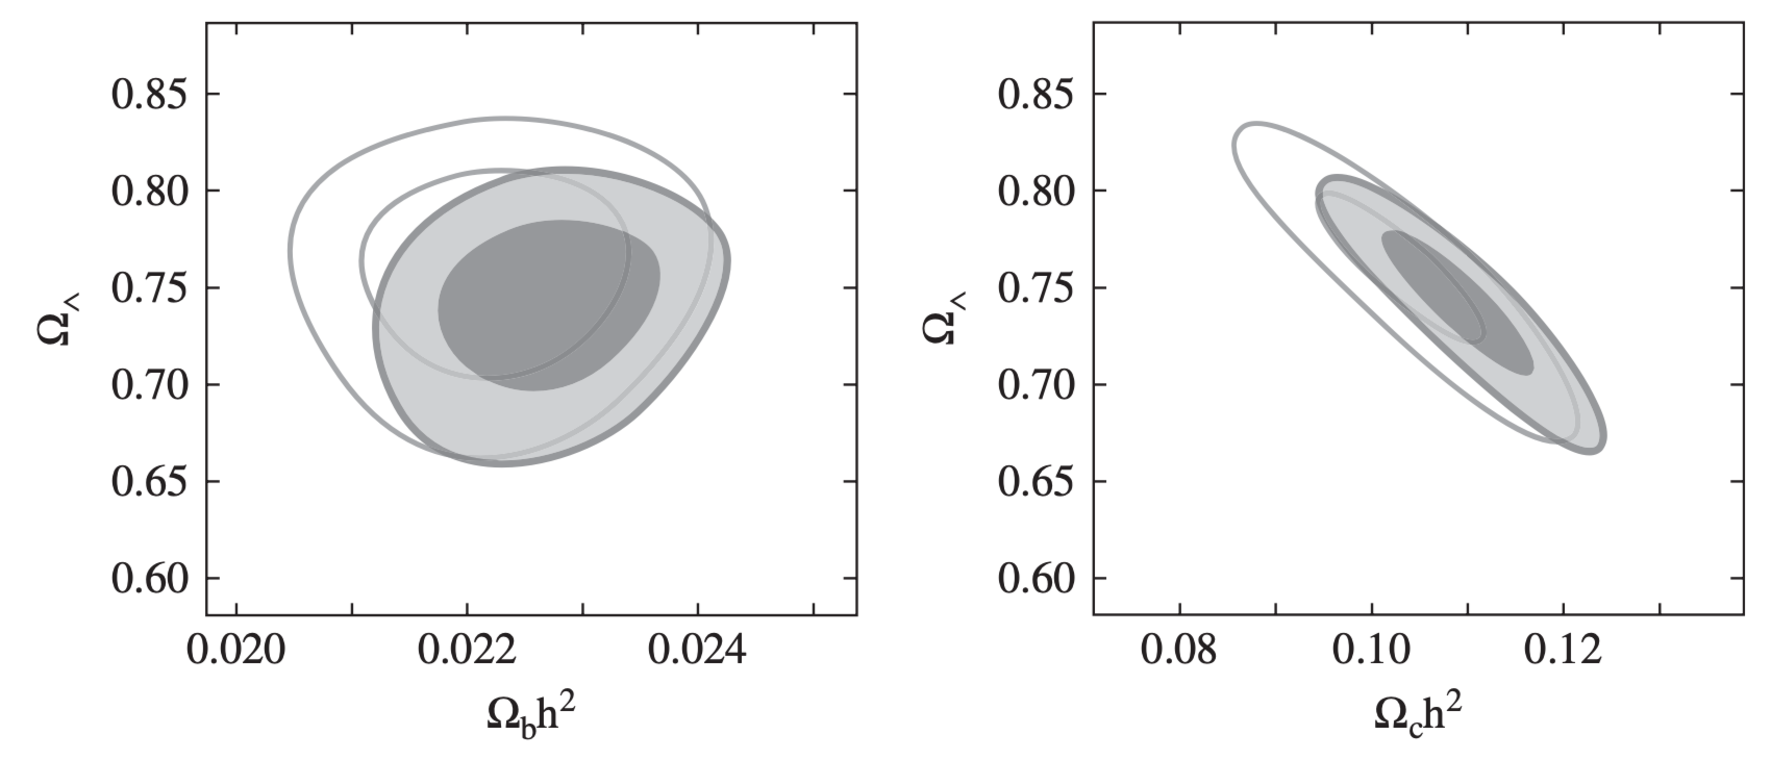
\includegraphics[scale=0.5]{DE-MCMC.pdf}
    \caption{Constraints on the free parameters of the $\Lambda$CDM
      model predicting a range of values for \(\Omega_{\Lambda}\). The contour 
      lines of each parameter represent confidence intervals in the 
      measurement. The values for \(\Omega_{\Lambda}\) are projected from
      Monte Carlo simulations of inputs from Wilkinson Microwave Anisotropy
      Probe data across the parameter space (\cite{Bennett_2011}).
      For inputs in the domain of likely values for \(\Omega_b\) and 
      \(\Omega_c\) seems to agree at \(\Omega_{\Lambda} \approx 0.73\).
    Credit: \cite{liddle2015introduction}}
    \label{fig:DE-constraints}
    \end{centering}
  \end{figure}

  Alternatives to the $\Lambda$CDM standard model of cosmology include
  modifications to the equation of state for dark energy, assumed to have a
  constant value of \(w = \frac{P}{\rho c^2} = -1\) for modern epoch as the
  universe cools in $\Lambda$CDM. Instead, if the energy density is pegged
  to the grid of spacetime and is expressed as a pressure on volumes of
  vacuum that becomes more significant where the matter density drops, as it
  has in the current era, to a value of \(w = -\frac{1}{3}\). This model is 
  called ``quintessence,'' is considered to be distinct from any 
  cosmological constant, but with a similar effect on observations
  (\cite{PhysRevLett.80.1582}). 

  In this modification to $\Lambda$CDM the source of pressure from dark 
  energy being a latent scalar field coupled to the geometry of the universe, 
  resulting in spacetime growth under a \(R_h = ct\) model 
  (\cite{10.1093/mnras/stv3012}), and is currently the best fit to observation 
  when compared across models and input parameters 
  (\cite{10.1093/mnras/sty1962}).

% 5. Growth of structure. [24]
% Describe how initial fluctuations from inflation have grown to form galaxies. 
% Consider the growth rate on various scales, and the different behaviour of 
% dark matter and baryons.  Include two figures for this section. 
\section{Growth of Structure}

  Galaxies and clusters of galaxies are the largest gravitationally
  bound structures seen in the universe. Because a galaxy is a bound object,
  it may be assumed to have not changed size with cosmological inflation,
  and so would have the same size today as prior to when \(\Omega_{\Lambda}\)
  dominated the energy budget. The era that separated one galaxy from the 
  constant background density of the universe occurred at redshift of 100.

  The model for collapse of the background density into a bound, virialized
  structure is the Jeans criteria for gravitational collapse. This model
  is highly dependent on the thermal velocity and mass density of a fluid
  (\cite{Jeans1902}).

  \begin{figure}[H]
    \begin{centering}
    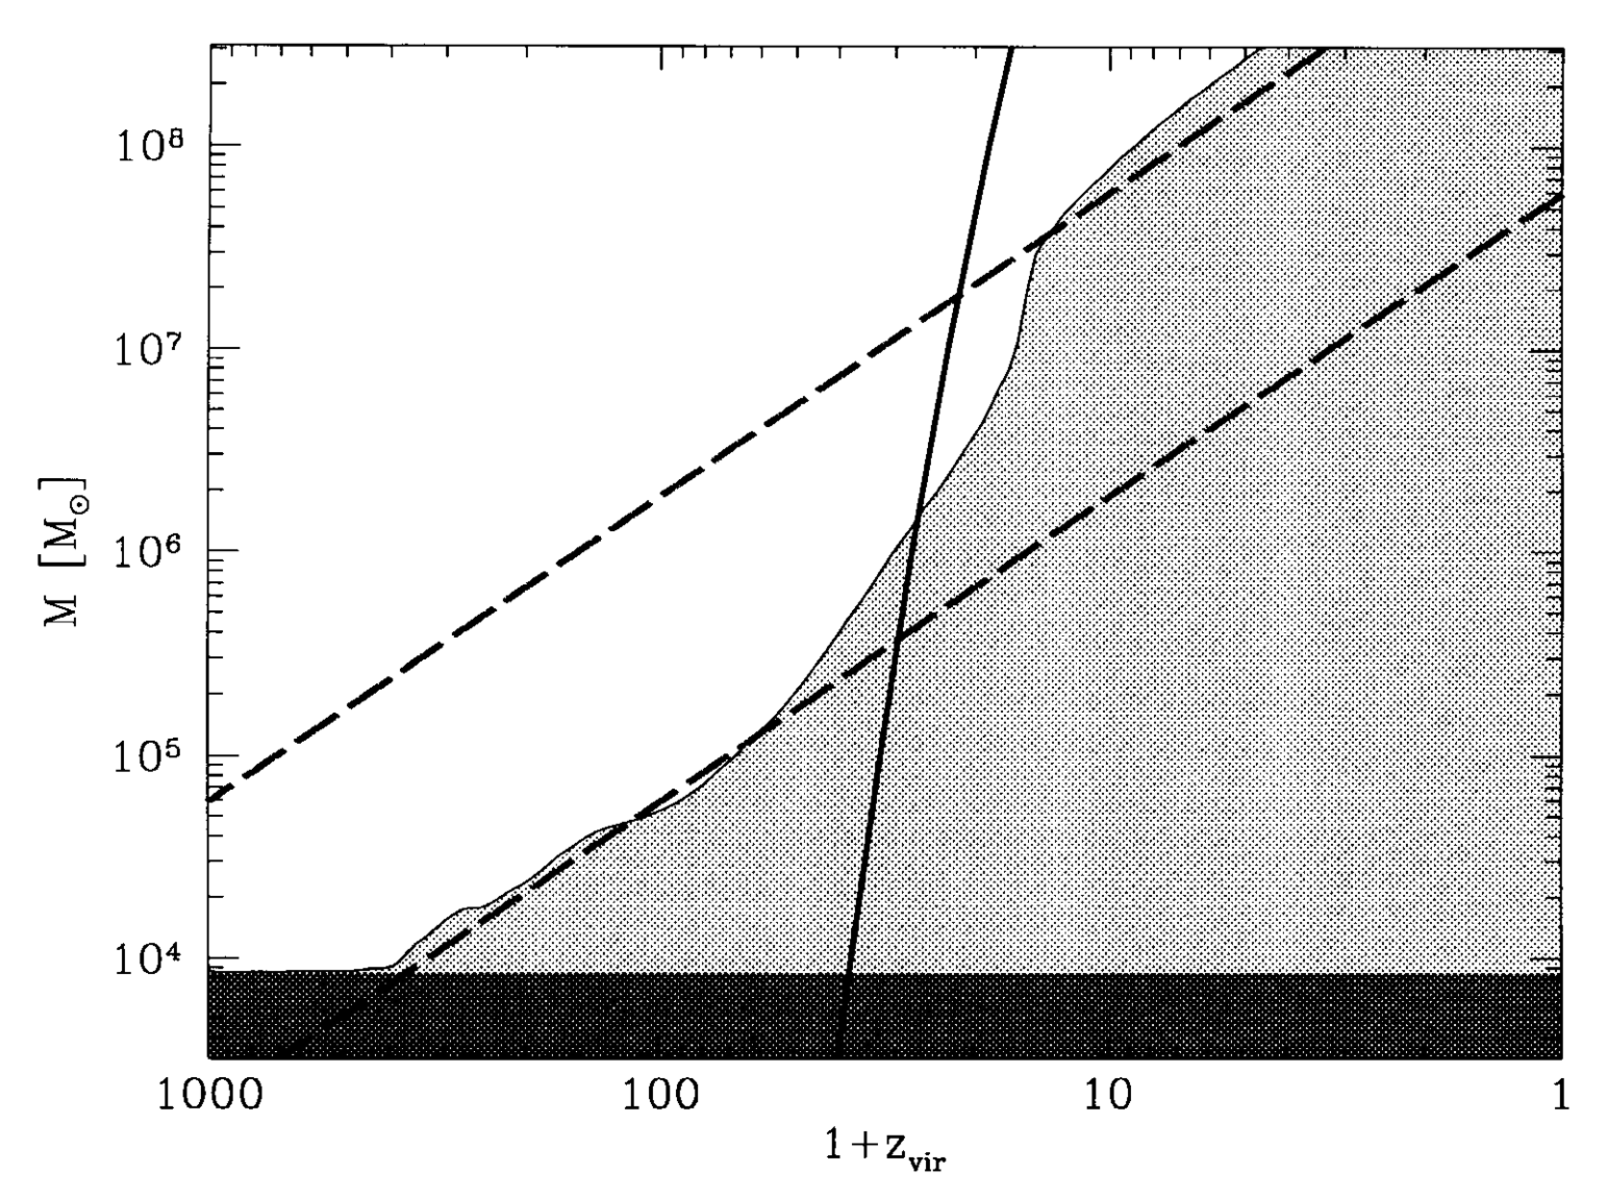
\includegraphics[scale=0.5]{Struct-mass.pdf}
    \caption{A graph of the minimum mass needed to collapse into a virialized
      structure. Masses greater than the shaded region can collapse; masses in 
      the light region can become luminous. The dashed lines represent 
      constant post-virialization temperatures of \SI{E4}{K} and \SI{E3}{K}. 
      The darkest shaded region cannot cool through radiative means because 
      the temperature after virializing would be the same as the cosmic 
      microwave background. The solid line is drawn to show about where 
      \(\Omega_b \times \SI{2E6}{M_{\astrosun}}\) can collapse at \(z=30\).
    Credit: \cite{1997ApJ...474....1T}}
    \label{fig:Struct-mass}
    \end{centering}
  \end{figure}

  The minimum mass for gravitational collapse after the radiation dominated
  era, with an initial temperature of \(T \approx \SI{3000}{K}\), is on the 
  order of \SI{E5}{M_{\astrosun}}, lower than the masses of galaxies and about 
  the mass similar to globular clusters, once hypothesized as the original
  structures formed after decoupling. The abundances of heavy elements found
  the spectra of globular clusters indicates more stellar processing than 
  could have occurred were globular clusters the original stellar population
  after the radiation era (\cite{Kalirai_2010}). The Jeans criteria indicates 
  that galactic masses could have coalesced into virialized structures since
  decoupling.

  The photon-baryon plasma fluid of the early universe was concurrent with
  a field of dark matter particles that, through fluctuations in its density 
  distribution, created the initial seeds for structural growth. The plasma
  was not coupled to the dark matter other than through gravitation. This
  caused a feedback loop in the evolution of the fields. While the photons 
  and ionized, relativistic atoms were coupled through electro-magnetic 
  interactions, causing a smoothness in the energy density of the plasma. This 
  enforced smoothness prevented the plasma from accreting into the 
  gravitational potentials of the dark matter. In turn, the dark matter could 
  not further collapse deeper into the potential wells as the plasma smoothed 
  out perturbations in the gravitational potential during the radiation era.

  This smoothing effect is Silk damping, which operates on multipole
  angular moments, \(l \approx 800\), a small scale among the anisotropy. 
  The mass within this scale was of order \SI{E13}{M_{\astrosun}}

  Two thermodynamic, baryonic models were developed to explain how the plasma 
  fluid would have evolved through the radiation dominated era. Hierarchical
  formation assumes an adiabatic fluid in which large scale structure formed
  first, splitting into smaller scale structures. An alternative formation
  begins with structure on small scales that grows into larger structures, 
  which requires that the radiation coupled to baryonic matter isothermally
  accrete into the local gravitational potentials within fluctations without 
  damping accretion. Both models require longer timescales than masses have
  been allowed since decoupling to become luminous galaxies, and so there
  must be a dark matter component to density fluctuations.

%behavior of dark matter halos accreting baryonic test particles
  Fig. \ref{fig:Struct-halo_accretion} is a hydrodynamic simulation of many 
  test particles of large masses clustering around dark matter halos. The
  Millennium Simulation found that nearly 50\% of baryonic test particles
  gravitated to halo seeds within the detectable threshold.
  (\cite{2005Natur.435..629S})

  \begin{figure}[H]
    \begin{centering}
    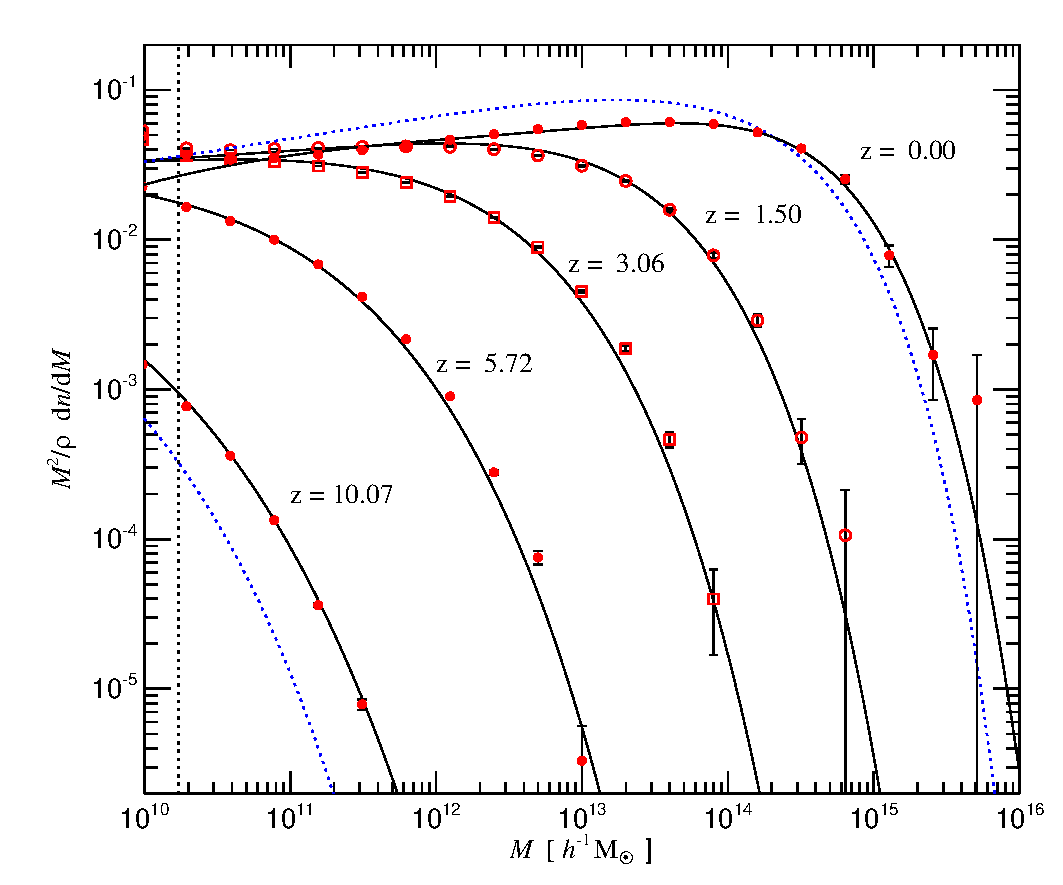
\includegraphics[scale=0.7]{Struct-halo_accretion.pdf}
    \caption{A Millennium Simulation generated co-moving number density of 
      dark matter halos, on the vertical axis, around which baryonic test
      particles of high mass, on the horizontal axis, are gravitating. The
      mass function of halos is given for different redshifts. The dotted
      lines are the similar, analytic Press–Schechter model.  This simulation 
      is regarded as extremely qualitatively similar to the outcome of 
      structural development in the real universe 
      (\cite{desjacques2018large}).
    Credit: \cite{2005Natur.435..629S}}
    \label{fig:Struct-halo_accretion}
    \end{centering}
  \end{figure}
  
  % The correlation function of galaxies and galaxy clusters is not the same,
  % which indicates that neither is an unbiased tracer of matter density
  % fluctuations in general (\cite{desjacques2018large}).

% 6. Conclusions.
% Providing some concluding remarks and briefly comment on future tests of 
% the standard model.
\section{Conclusions}
  The Standard Model of Cosmology explains how much of the fossil evidence
  of a Hot Big Bang came to be, the features embedded in the cosmic microwave 
  background anisotropy and the abundances of primordial elements in a 
  universe that is the undergoing further nuclear processing. Dark matter
  and dark energy have an unexplained origin in the current theory.

  Primordial black holes are a potential MACHO candidate for dark matter, 
  and may be a source of SNe Type 1a (\cite{PhysRevD.92.063007}), but their
  existence may be exclusive of WIMPs (\cite{Adamek_2019}). 

  Data from the Planck mission may indicate that universe has a closed 
  geometry after all, which challenges the inflation solution for the horizon
  and flatness problems (\cite{2020NatAs...4..196D}). Resolving the 
  curvature of spacetime is a fundamental test of validity.

  The validity of $\Lambda$CDM requires accounting for the dark sources of
  energy density in a way that satisfies the model. Disagreement with
  fundamental assumptions, such as about the flatness of the universe,
  also should be reconfirmed.

% Constraining the free parameters of the physics of the Standard Model to
% fit the best observations of the universe today produces a benchmark model,
% which can be broken down into contributions of different 
% constituents to the energy density of the unverse in the following way,
% (\cite{ryden2003introduction}):

% \begin{center}
% \begin{tabular}{ c c c }
%   Photons & \(\Omega_{\gamma} = 5.35E-5 \) \\
%   Neutrinos & \(\Omega_{\nu} = 3.65E-5 \) \\
%   Total radiation & \(\Omega_{r} = 9.0E-5 \) \\
%   Baryonic matter & \(\Omega_{b} = 0.048 \) \\
%   Nonbaryonic matter & \(\Omega_{dm} = 0.262 \) \\
%   Total matter & \(\Omega_{m} = 0.31 \) \\
%   Cosmological constant & \(\Omega_{\Lambda} \approx 0.69 \)
%\end{tabular}
%\end{center}

%TC:ignore

\pagebreak
\begin{singlespace}
\printbibliography
\end{singlespace}

%TC:endignore

\end{document}

